\documentclass{beamer}

% Encoding & language
\usepackage[T1]{fontenc}
\usepackage[utf8]{inputenc}
\usepackage[english]{babel}
\usepackage{transparent}

% Bibliography
\usepackage[numbers]{natbib}
\bibliographystyle{ieeetr}

% Figures, tables, colors
\usepackage{graphicx}
\usepackage{subcaption}
\usepackage{tabularx}
\usepackage{booktabs}
\usepackage{multirow}
\usepackage{makecell}
\usepackage[table, svgnames]{xcolor}

\usepackage{caption}
\captionsetup[table]{justification=centering}

% Beamer
\setbeamerfont{framesubtitle}{size=\normalsize}

% Misc
\usepackage{amsmath}
\usepackage{amssymb}
\usepackage{hyperref}
\usepackage{tikz}
\usetikzlibrary{arrows.meta, positioning, calc}
\DeclareMathOperator{\jinc}{jinc}

% Section.slide numbering in frame titles (e.g. "2.3")
\newcounter{sframe}[section]
\renewcommand{\thesframe}{\thesection.\arabic{sframe}}
\newcommand{\ftitle}[1]{\stepcounter{sframe}{\normalsize\thesframe}\quad #1}

% Transparent, Checkmark
\usepackage{transparent}
\newcommand{\dimtxt}[1]{{\transparent{0.25}#1}} % 0.25-0.45
\usepackage{pifont}
\newcommand{\cmark}{\ding{51}}
\newcommand{\xmark}{\ding{55}}

\mode<presentation>{
  \usetheme{Madrid}
  \usecolortheme{default}
  \setbeamertemplate{caption}[numbered]
  % Bad projector in the defense room: maximize usable width so
  % tables, axes, and tick labels are as large as possible.
  \setbeamersize{text margin left=0.35cm, text margin right=0.35cm}
}

\title[Solar Radio Interferometer Simulation]{%
  {\Large\bfseries End-to-End Simulation of a Four-Element UHF Radio\\
  Interferometer for Solar Radio Observation at 610~MHz}%
}

\subtitle{Graduation Thesis Defense}

\author[N. B. Quan]
{Nguyen Ba Quan (20224350) \\ Supervisor: Assoc.\ Prof.\ Dr.\ Ha Duyen Trung}

\institute[SEEE--HUST]
{
School of Electrical and Electronic Engineering \\
Hanoi University of Science and Technology
}

\date{\today}

\setbeamertemplate{bibliography item}{\insertbiblabel}

\begin{document}

% ============================================================
% Title
\begin{frame}
  \titlepage
\end{frame}

\begin{frame}{Outline}
\tableofcontents
\end{frame}

% ============================================================
\section{Motivation}

\begin{frame}{\ftitle{Motivation: Why Monitor Solar Radio Bursts}}
\begin{columns}[c]
\column{.46\textwidth}
\centering
\scriptsize
\colorbox{blue!8}{\parbox{.92\linewidth}{\centering Solar flares \&
coronal mass ejections $\to$ \textbf{solar radio bursts}}}\\[3pt]
$\Downarrow$\\[3pt]
\colorbox{blue!8}{\parbox{.92\linewidth}{\centering Changes the
ionosphere's electron density}}\\[3pt]
$\Downarrow$\\[3pt]
\colorbox{orange!15}{\parbox{.92\linewidth}{\centering Disturbs
electronic devices --- e.g.\ \textbf{2022 Starlink}: 38/49 satellites
lost to a geomagnetic storm~\cite{berger2023starlink}}}\\[3pt]
$\Downarrow$\\[3pt]
\colorbox{green!15}{\parbox{.92\linewidth}{\centering $\Rightarrow$
Ground-based radio observation gives \textbf{1--3 days} of early
warning}}
\column{.5\textwidth}
\centering
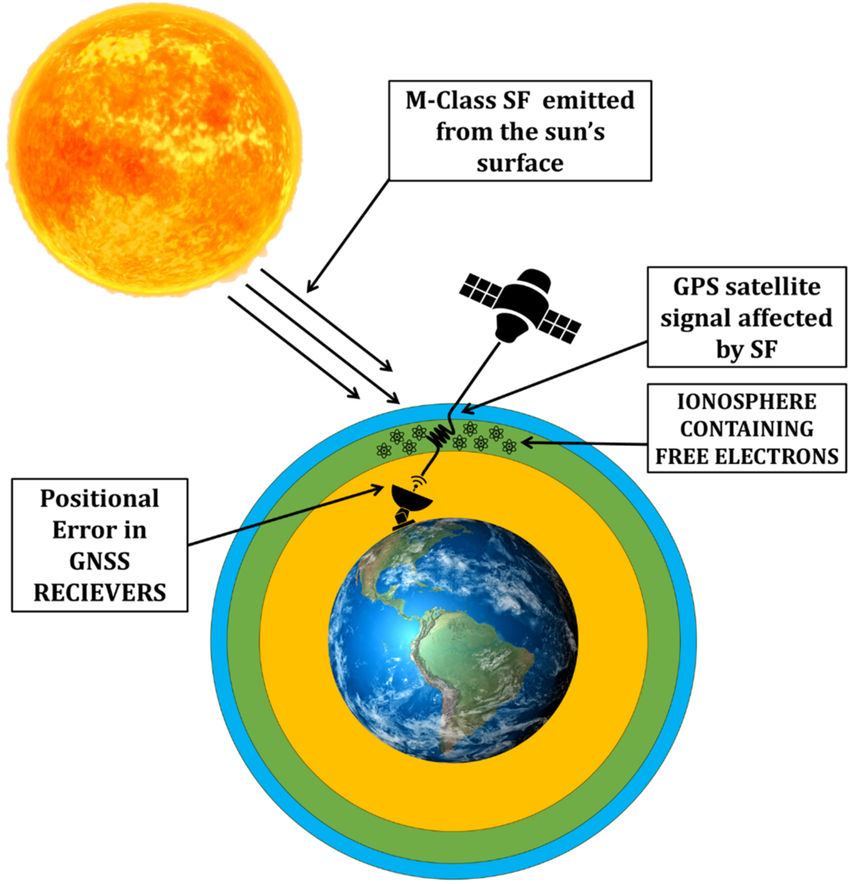
\includegraphics[width=\linewidth]{figs/fig_gnss_ionosphere.png}
\end{columns}
\vspace{4pt}
\centering
\small Fig.~1. How solar radio bursts affect our electronic devices.
\scriptsize Transient Type~II/III bursts can raise the quiet-Sun flux by
$10^{4}$--$10^{5}\times$ --- full burst classification in backup.
\end{frame}

\begin{frame}{\ftitle{Big Dish vs.\ Aperture Synthesis}}
\centering
\begin{columns}[t]
\column{.24\textwidth}
\centering
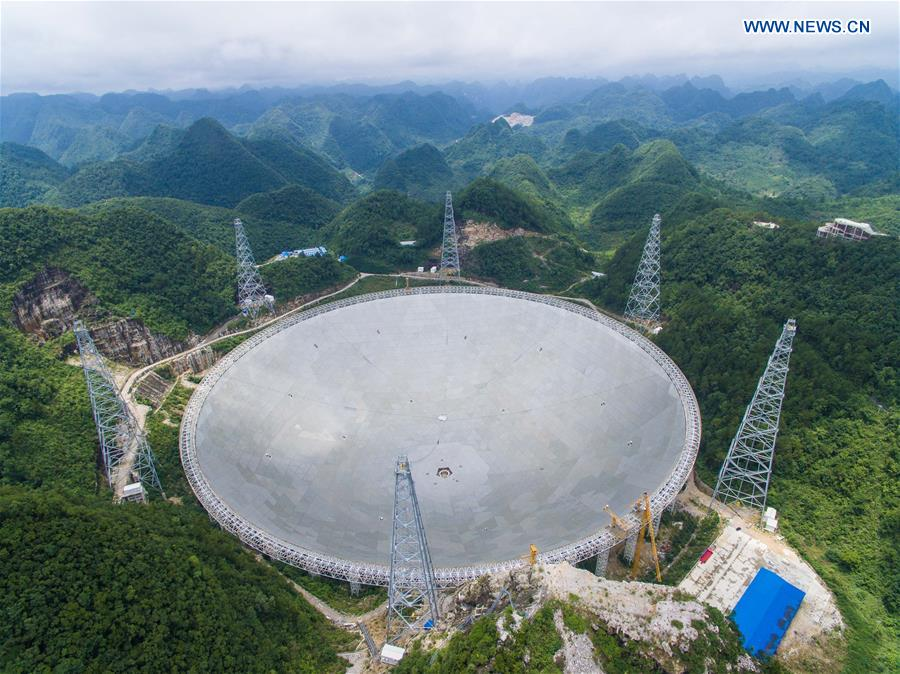
\includegraphics[width=.42\linewidth]{figs/photo_fast_dish.jpg}\\
\scriptsize Fig.~2. FAST, China.
\column{.24\textwidth}
\centering
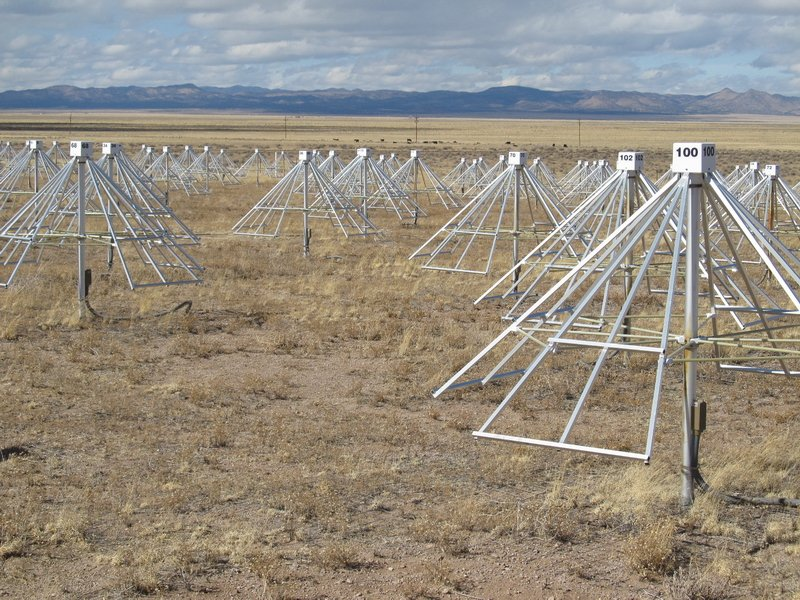
\includegraphics[width=.42\linewidth]{figs/photo_dlite_array.jpg}\\
\scriptsize Fig.~3. DLITE, USA.
\end{columns}
\centering
\scalebox{0.94}{%
\scriptsize
\renewcommand{\arraystretch}{1.05}
\setlength{\tabcolsep}{3pt}
\begin{tabular}{@{}l|p{2.35cm}p{2.35cm}|p{2.35cm}p{2.35cm}@{}}
\toprule
 & \multicolumn{2}{c|}{\textbf{Big Dish (FAST)}} &
 \multicolumn{2}{c}{\textbf{Aperture Synthesis (this thesis)}} \\
\textbf{Criterion} & \cellcolor{green!15}\cmark & \cellcolor{red!10}\xmark
 & \cellcolor{green!15}\cmark & \cellcolor{red!10}\xmark \\
\midrule
Resolution &
\cellcolor{green!5}--- &
\cellcolor{red!4}Capped $\approx$500~m --- physically cannot grow &
\cellcolor{green!5}$\propto$ longest baseline (km-scale) &
\cellcolor{red!4}Needs many antennas $+$ full rotation synthesis \\
Cost &
\cellcolor{green!5}Known, one-off &
\cellcolor{red!4}Hundreds of millions of \$ &
\cellcolor{green!5}$\approx$\$1000s per antenna &
\cellcolor{red!4}More antennas $\Rightarrow$ more receiver chains \\
Upgrade path &
\cellcolor{green!5}--- &
\cellcolor{red!4}Frozen once built &
\cellcolor{green!5}Just move or add antennas &
\cellcolor{red!4}--- \\
Signal complexity &
\cellcolor{green!5}Simple: one receiver, no combining &
\cellcolor{red!4}--- &
\cellcolor{green!5}--- &
\cellcolor{red!4}Must combine signals phase-coherently \\
\bottomrule
\end{tabular}%
}
\vspace{2pt}

\begin{alertblock}{\centering Bottom line}
\centering\scriptsize Same resolution goal, opposite price: the big
dish pays in \textbf{concrete and steel}; aperture synthesis pays in
\textbf{antennas and signal-processing complexity} --- exactly what this
thesis simulates and validates.
\end{alertblock}
\end{frame}

\begin{frame}{\ftitle{Objectives}}
\vspace{-10pt}
\begin{columns}[t]
\column{.34\textwidth}
\centering
\mbox{}\\[22pt]
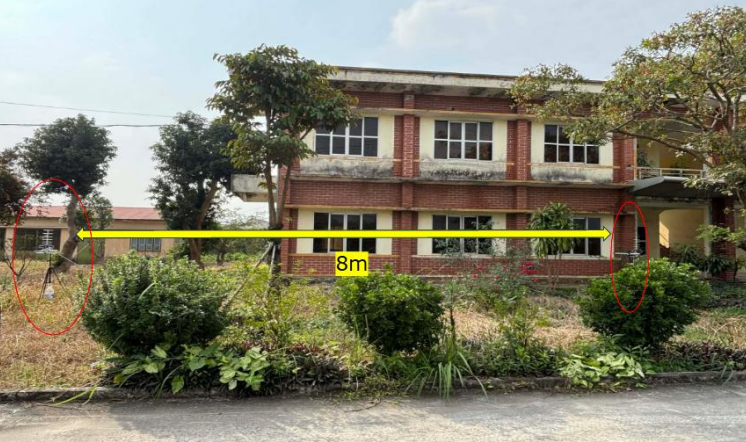
\includegraphics[width=.75\linewidth]{figs/photo_xuan_mai_field.png}\\
\scriptsize Fig.~4. Xuan Mai field trial: 2-element Yagi-Uda, 8~m baseline.
\column{.62\textwidth}
\scriptsize
\begin{itemize}
  \setlength{\itemsep}{2pt}
  \item A previous 2-antenna field trial at Xuan Mai gave only an
  \textbf{ambiguous day/night trend} --- no clear interference fringes,
  and no way to tell which part of the hardware was at fault just by
  inspection.
  \item This thesis builds and validates an end-to-end simulation, then
  uses it to \textbf{diagnose the exact cause} of that failure ---
  quantified with real numbers and a concrete hardware fix in the
  results.
\end{itemize}
\end{columns}
\vspace{3pt}
\centering
\textbf{Two objectives}
\vspace{-3pt}

\begin{columns}[t]
\column{.48\textwidth}
\begin{block}{Build a trustworthy physics simulation}
\centering
\scriptsize Signal $\to$ correlator $\to$ image. Validated against
classical theory and real hardware, so it can safely stand in before
expensive field testing.
\end{block}
\column{.48\textwidth}
\begin{block}{Optimize antenna placement (array geometry)}
\centering
\scriptsize Use that simulator to search many array layouts. Find
which placement of the same antennas gives the best 2-D resolution,
without buying more hardware.
\end{block}
\end{columns}
\end{frame}

% ============================================================
\section{Method}

\begin{frame}{\ftitle{Simulation Pipeline: From Flux to Image}}
\centering
\scalebox{0.92}{%
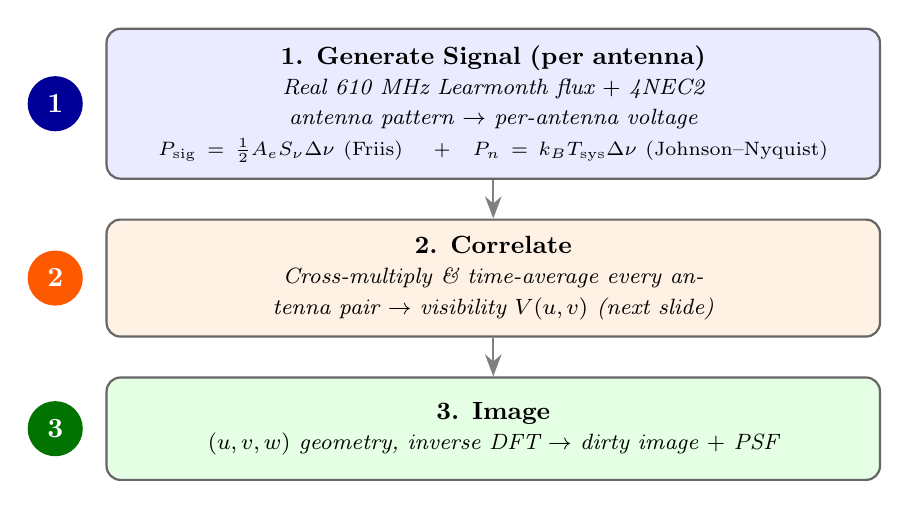
\begin{tikzpicture}[
  badge/.style={circle, fill=blue!60!black, text=white, font=\bfseries,
                minimum size=0.7cm, inner sep=0pt},
  proc/.style={rectangle, rounded corners=5pt, draw=black!60, thick,
               text width=9.4cm, align=center, inner sep=6pt,
               minimum height=1.3cm, font=\small},
  arr/.style={-{Stealth[length=8pt]}, thick, black!50}
]
\node[proc, fill=blue!8] (gen) {\textbf{1. Generate Signal (per antenna)}\\
{\footnotesize\itshape Real 610~MHz Learmonth flux $+$ 4NEC2 antenna
pattern $\to$ per-antenna voltage}\\
{\scriptsize$P_{\rm sig}=\tfrac12 A_eS_\nu\Delta\nu$ (Friis) $\quad+\quad
P_n=k_BT_{\rm sys}\Delta\nu$ (Johnson--Nyquist)}};
\node[badge, left=8pt of gen] {1};
\node[proc, fill=orange!10, below=14pt of gen] (corr) {\textbf{2. Correlate}\\{\footnotesize\itshape Cross-multiply \& time-average every antenna pair $\to$ visibility $V(u,v)$ (next slide)}};
\node[badge, fill=orange!70!red, left=8pt of corr] {2};
\node[proc, fill=green!10, below=14pt of corr] (img) {\textbf{3. Image}\\{\footnotesize\itshape $(u,v,w)$ geometry, inverse DFT $\to$ dirty image $+$ PSF}};
\node[badge, fill=green!45!black, left=8pt of img] {3};
\draw[arr] (gen) -- (corr);
\draw[arr] (corr) -- (img);
\end{tikzpicture}%
}

\vspace{6pt}
\small $\Rightarrow$ This same three-box chain is re-run for every
candidate antenna layout --- comparing those outputs is the second half
of the thesis.
\end{frame}

\begin{frame}{\ftitle{What Is a Visibility?}}
\begin{columns}[c]
\column{.58\textwidth}
\centering
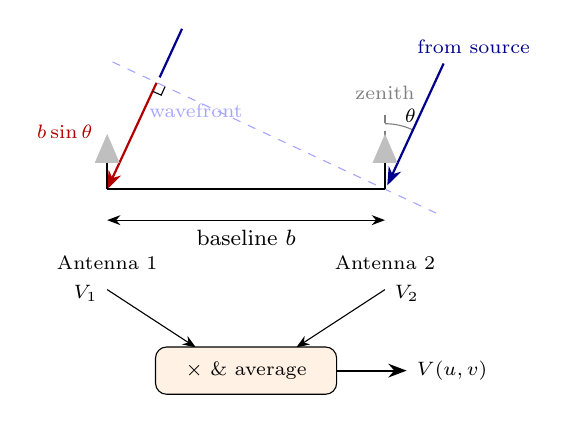
\begin{tikzpicture}[scale=0.98, >=Stealth, font=\footnotesize]
% short vertical reference tick at antenna 2 (zenith direction), kept small
% so it doesn't compete visually with the wavefront label
\draw[dashed, gray] (3.6,0) -- (3.6,1.05);
\node[gray] at (3.6,1.25) {\scriptsize zenith};
\draw[gray] (3.6,0.85) arc[start angle=90, end angle=65, radius=0.85];
\node at (3.93,0.95) {\scriptsize $\theta$};
% two PARALLEL rays from the same distant source (far field: same direction
% arrives at both antennas) -- antenna 2's ray reaches the wavefront first
\draw[->, thick, blue!55!black] (4.36,1.63) -- (3.63,0.05);
\node[blue!55!black] at (4.75,1.85) {\scriptsize from source};
\draw[thick, blue!55!black] (0.97,2.08) -- (0.68,1.45);
% wavefront: the line of constant phase that has just reached antenna 2,
% extended to show where it crosses antenna 1's own ray (point F)
\draw[dashed, blue!35] (0.07,1.65) -- (4.33,-0.34);
\node[blue!35] at (1.15,1.02) {\scriptsize wavefront};
% extra path antenna 1's ray must still cover, along the SAME ray direction,
% from the wavefront-crossing point F down to antenna 1 -- this is b sin(theta)
\draw[thick, red!70!black, ->] (0.64,1.38) -- (0,0);
\node[red!70!black] at (-0.55,0.75) {\scriptsize $b\sin\theta$};
% right-angle marker at F (ray direction is perpendicular to the wavefront)
\draw (0.59,1.27) -- (0.70,1.22) -- (0.75,1.33);
% baseline
\draw[thick] (0,0) -- (3.6,0);
\draw[<->] (0,-0.4) -- (3.6,-0.4) node[midway, below]{baseline $b$};
% antenna icons
\draw[thick] (0,0) -- (0,0.35);
\filldraw[gray!50] (-0.15,0.35) -- (0.15,0.35) -- (0,0.7) -- cycle;
\draw[thick] (3.6,0) -- (3.6,0.35);
\filldraw[gray!50] (3.45,0.35) -- (3.75,0.35) -- (3.6,0.7) -- cycle;
\node at (0,-0.95) {\scriptsize Antenna 1};
\node at (3.6,-0.95) {\scriptsize Antenna 2};
% multiply & average box
\draw[->] (0,-1.3) -- (1.15,-2.05);
\node[left] at (0,-1.35) {\scriptsize $V_1$};
\draw[->] (3.6,-1.3) -- (2.45,-2.05);
\node[right] at (3.6,-1.35) {\scriptsize $V_2$};
\node[draw, rounded corners, fill=orange!10, minimum width=2.3cm,
      minimum height=0.6cm] (mult) at (1.8,-2.35) {\scriptsize $\times$ \&
      average};
\draw[->, thick] (mult.east) -- ++(0.9,0) node[right]{\scriptsize $V(u,v)$};
\end{tikzpicture}
\column{.38\textwidth}
\footnotesize
\begin{itemize}
  \setlength{\itemsep}{3pt}
  \item Each antenna pair measures one geometric delay
  $\tau=b\sin\theta/c$ $\Rightarrow$ the correlator collapses it to
  \textbf{one complex number}, a \textbf{visibility}: one interference
  fringe on the sky.
  \item Earth's rotation changes $\theta$ through the day
  $\Rightarrow$ the correlator output oscillates --- the measurable
  \textbf{fringe}.
  \item Each baseline is one spatial frequency; many baselines
  $\Rightarrow$ many Fourier components, combined into an image
  (\textbf{van Cittert--Zernike theorem}).
\end{itemize}
\end{columns}
\end{frame}

% ============================================================
\section{Antenna \& Setup}

\begin{frame}{\ftitle{Antenna: A Validated Model}}
\begin{columns}[c]
\column{.42\textwidth}
\centering
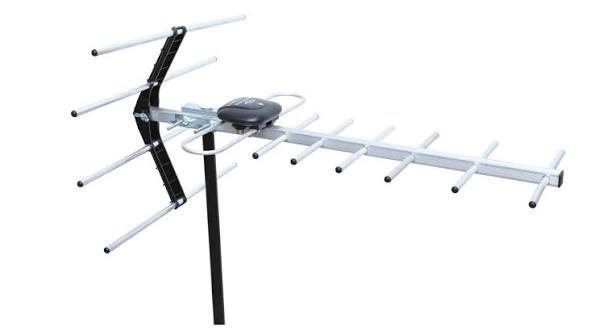
\includegraphics[width=.68\linewidth]{figs/photo_hkd_antenna.jpg}\\
\scriptsize Commercial HKD~G11KD-T2 Yagi-Uda, modelled wire-by-wire in
4NEC2~\cite{nec2}.
\begin{table}
\small
\centering
\begin{tabular}{lc}
\toprule
\textbf{Quantity} & \textbf{Value} \\
\midrule
Input $Z$ & $108.4 - j22.0\;\Omega$ \\
Forward gain & 9.48 dBi \\
HPBW & $\approx 52^\circ$ \\
SWR (75~$\Omega$) & 1.55 \\
\bottomrule
\end{tabular}
\end{table}
\column{.54\textwidth}
\begin{table}
\footnotesize
\centering
\begin{tabular}{lcc}
\toprule
\textbf{Method} & \textbf{SWR} & \makecell{\textbf{Return}\\\textbf{loss}} \\
\midrule
NanoVNA (measured) & 1.59 & $\approx-12.8$~dB \\
4NEC2 (simulated)  & 1.55 & $\approx-13.3$~dB \\
\bottomrule
\end{tabular}
\end{table}
\footnotesize
\begin{itemize}
  \item Measured and simulated impedance agree closely $\Rightarrow$ the
  simulated antenna pattern is trustworthy enough to drive the imaging
  pipeline.
  \item Mutual coupling falls below $-78$~dB by 5~m, $-87$~dB by 10~m
  $\Rightarrow$ antennas behave as \textbf{independent sensors} at every
  operating baseline used in this thesis (8~m and above).
\end{itemize}
\end{columns}
\end{frame}

\begin{frame}{\ftitle{Real Input Data}}
\centering
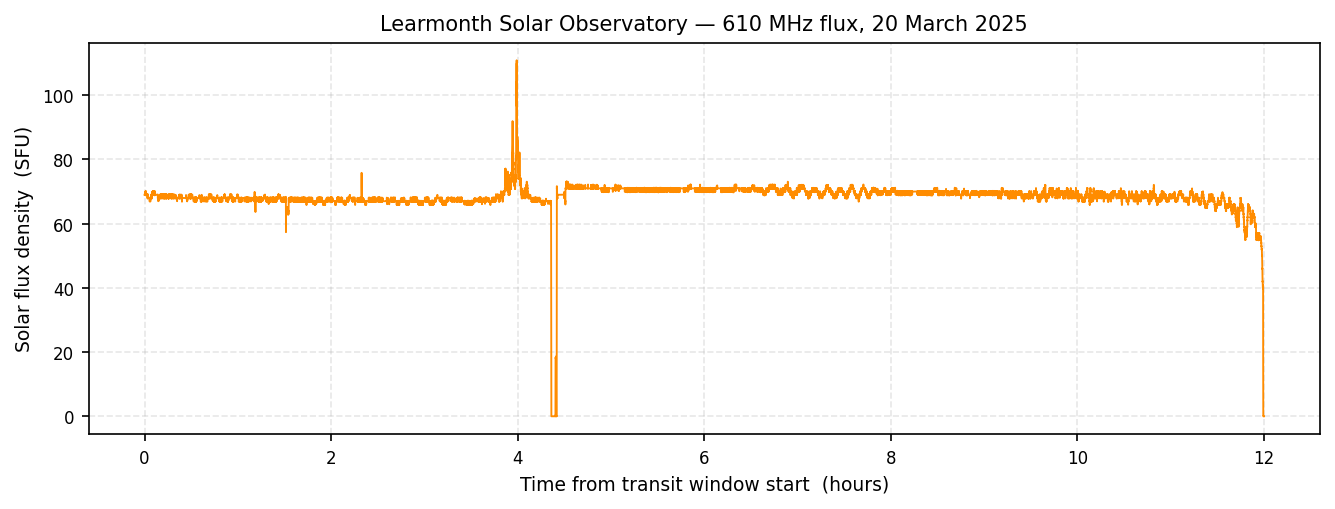
\includegraphics[width=0.78\linewidth]{figs/fig_sws_flux_day.png}

\vspace{4pt}
\footnotesize
Real, archived, already-calibrated 610~MHz flux from SWS Learmonth,
Australia~\cite{sws} (20~March~2025) --- the raw input, not re-simulated
internally.
\begin{itemize}
  \footnotesize
  \setlength{\itemsep}{1pt}
  \item Frequency 610~MHz, bandwidth 1~MHz, $T_{\rm sys}=150$~K
  (ideal receiver).
  \item Site: Learmonth Observatory, latitude $-22.2^\circ$.
  \item Baselines swept from 8~m to 130~m using the same 4-antenna
  hardware.
\end{itemize}
\end{frame}

% ============================================================
\section{Validation}

\begin{frame}{\ftitle{Visibility Validation: Fringe \& Jinc Curve}}
\centering
\begin{columns}[t]
\column{.48\textwidth}
\centering
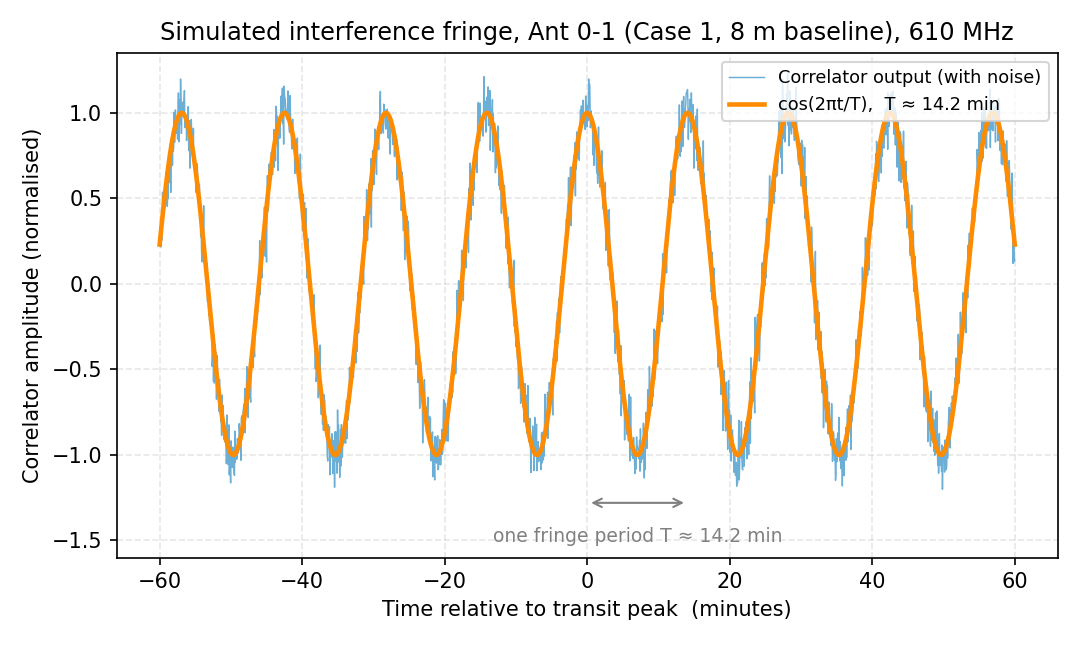
\includegraphics[width=\linewidth]{figs/fig_fringe_time_8m.png}\\
\footnotesize Fringe period $\approx$14~min on the 8~m adjacent-pair
baseline (Case~1), matching the analytic prediction for that baseline
and date.
\column{.48\textwidth}
\centering
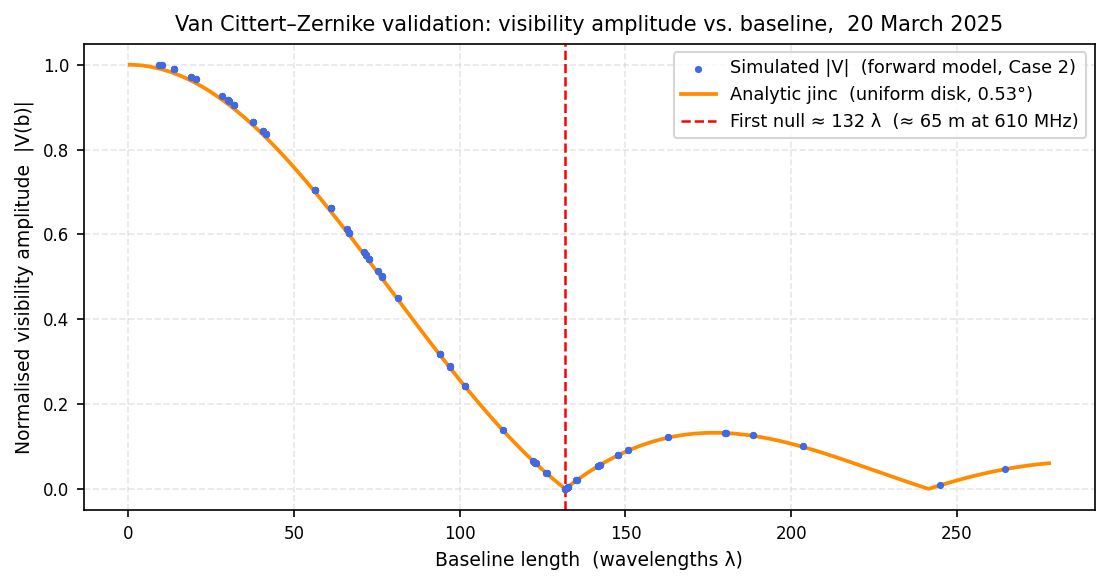
\includegraphics[width=\linewidth]{figs/fig_visibility_jinc.png}\\
\footnotesize Visibility amplitude falls on the analytic jinc curve for
a uniform solar disk; first null at $\approx130\,\lambda$.
\end{columns}
\vspace{8pt}
\small $\Rightarrow$ Two independent checks in the visibility domain,
both satisfied on real solar flux --- the correlator implements van
Cittert--Zernike correctly.
\end{frame}

\begin{frame}{\ftitle{Imaging Validation: Dirty Image $=$ Sky $\ast$ PSF}}
\centering
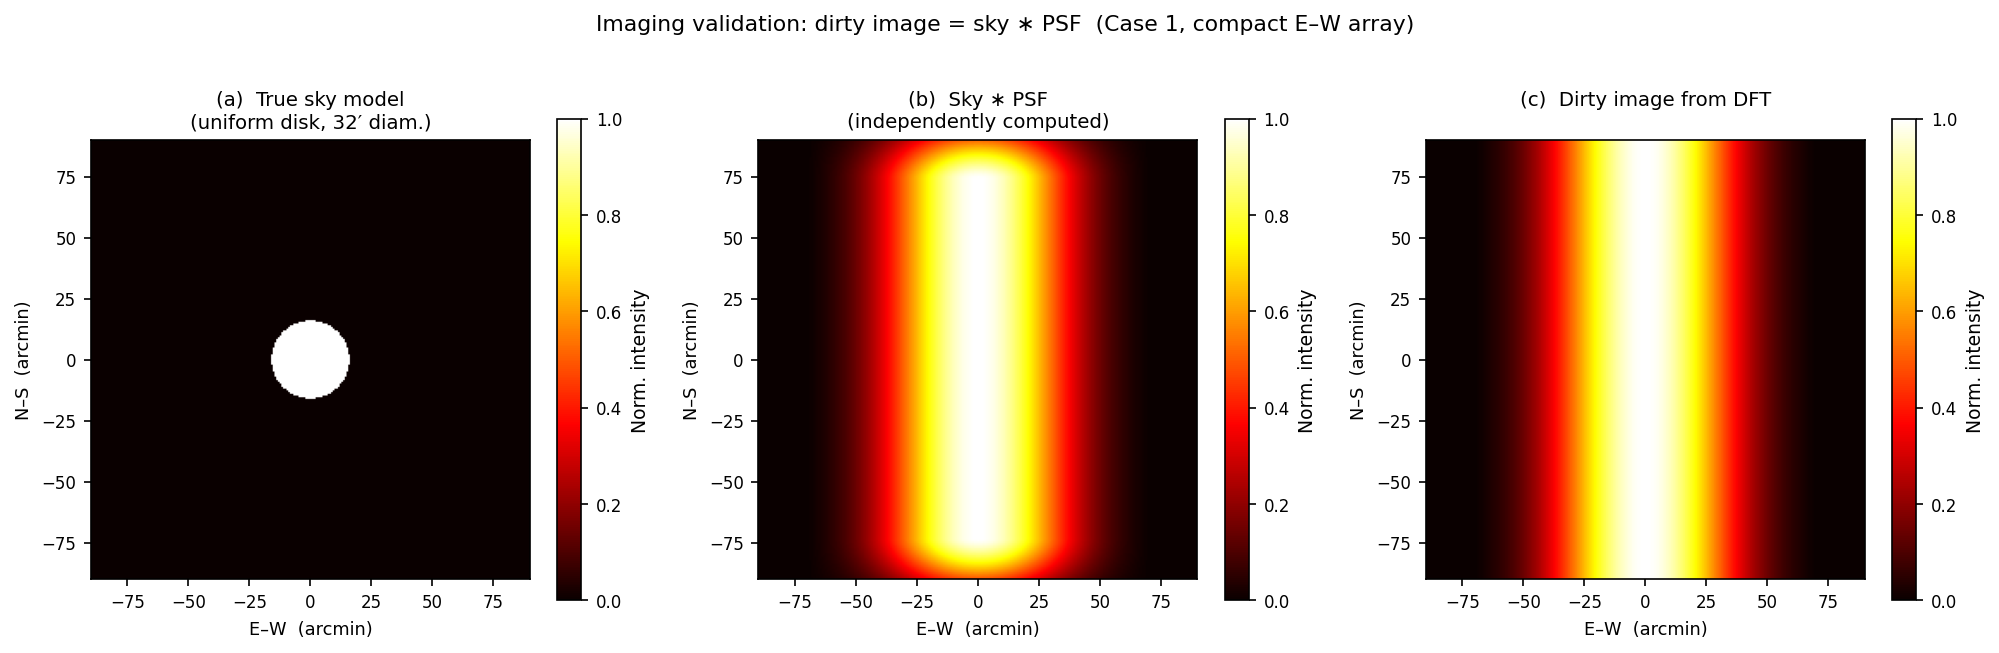
\includegraphics[width=0.85\linewidth]{figs/fig_sky_conv_psf.png}

\vspace{4pt}
\footnotesize (a) true sky $\ast$ (b) PSF $=$ (c) dirty image, computed
independently via gridding $+$ FFT --- (b) and (c) agree to
\textbf{machine precision}.
\vspace{8pt}

\small $\Rightarrow$ A third, independent check --- this time in the
imaging domain --- confirms the correlator, $(u,v)$-sampling, and
inverse DFT are all self-consistent, for \emph{any} 2-D array layout.
\end{frame}

% ============================================================
\section{Results}

\begin{frame}{\ftitle{Why Array Layout Matters}}
\centering
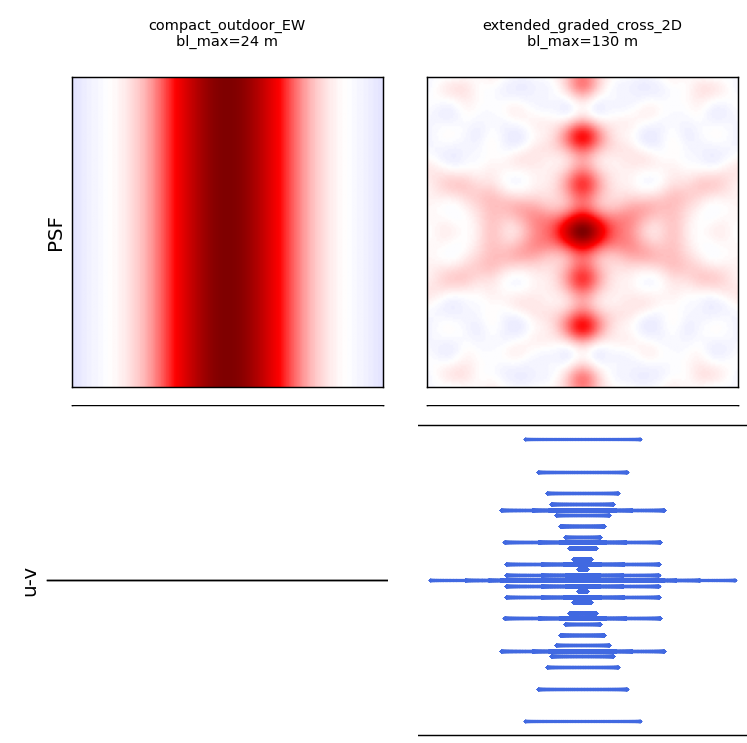
\includegraphics[width=0.46\linewidth]{figs/fig_layout_sweep_2col.png}

\footnotesize
\begin{itemize}
  \setlength{\itemsep}{0pt}
  \item Compact E--W: 1-D $(u,v)$ coverage only $\Rightarrow$ PSF is a
  single elongated stripe.
  \item A 2-D graded cross fills the $(u,v)$ plane in \textbf{both}
  directions $\Rightarrow$ PSF sidelobes drop by $\approx20$~dB vs.\
  compact E--W.
  \item[$\Rightarrow$] \textbf{2-D coverage} is what removes the
  sidelobes --- the next slide isolates this with a fixed 4-antenna
  budget.
\end{itemize}
\end{frame}

\begin{frame}{\ftitle{Array Geometry Comparison}}
\centering
\begin{minipage}{\linewidth}
\footnotesize
\renewcommand{\arraystretch}{1.0}
\setlength{\tabcolsep}{6pt}
\begin{tabular}{ccp{6.4cm}}
\toprule
\textbf{Layout} & \textbf{Dirty Image} & \textbf{Result} \\
\midrule
\parbox{1.9cm}{\centering
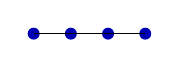
\begin{tikzpicture}[baseline=0pt, scale=1.35]
\foreach \x in {0,0.35,0.7,1.05} \fill[blue!70!black] (\x,0) circle (1.6pt);
\draw[thin] (0,0) -- (1.05,0);
\end{tikzpicture}\\[3pt]{\small E-W line, 24~m}} &
\parbox{2.3cm}{\centering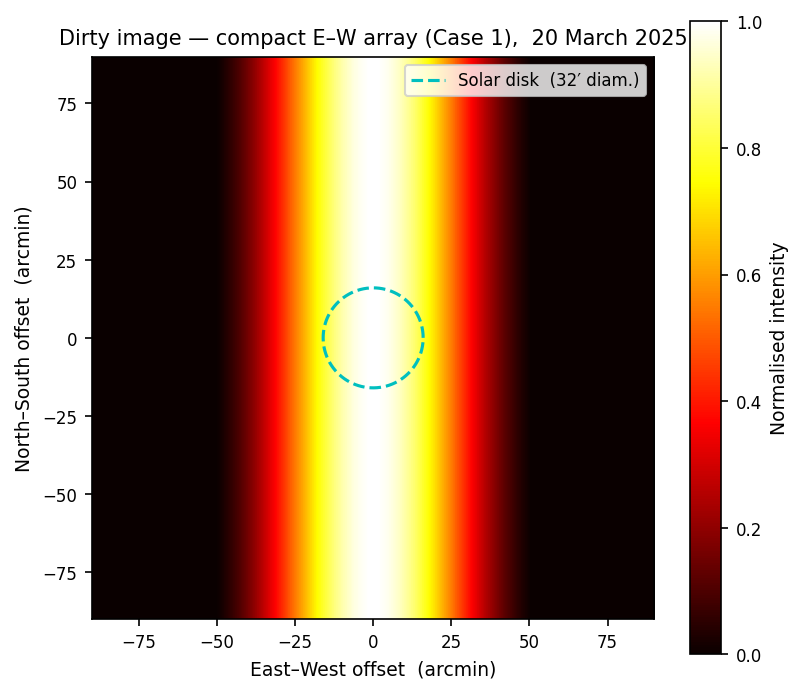
\includegraphics[width=\linewidth]{figs/fig_dirty_image.png}} &
\textbf{Case 1.} 1-D baselines only $\Rightarrow$ N-S FWHM $180.0'$ ---
smeared and unresolved in North-South. \\[2pt]

\parbox{1.9cm}{\centering
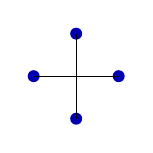
\begin{tikzpicture}[baseline=0pt, scale=1.35]
\fill[blue!70!black] (0,0.4) circle (1.6pt);
\fill[blue!70!black] (0,-0.4) circle (1.6pt);
\fill[blue!70!black] (0.4,0) circle (1.6pt);
\fill[blue!70!black] (-0.4,0) circle (1.6pt);
\draw[thin] (0,0.4) -- (0,-0.4);
\draw[thin] (-0.4,0) -- (0.4,0);
\end{tikzpicture}\\[3pt]{\small Cross, 8~m}} &
\parbox{2.3cm}{\centering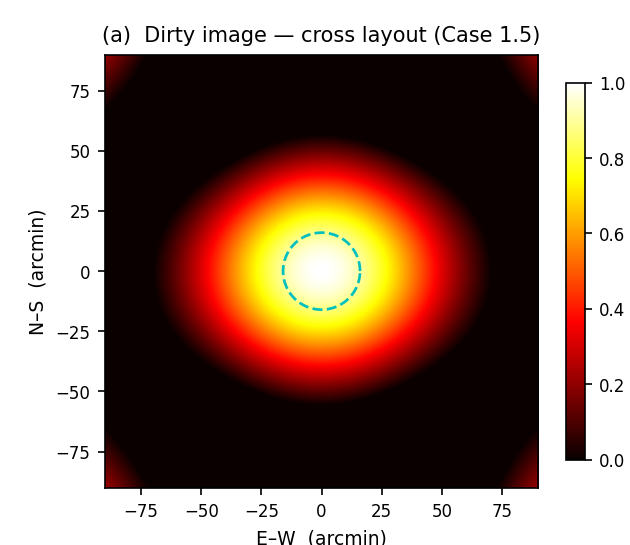
\includegraphics[width=\linewidth]{figs/fig_case15_dirty_crop.png}} &
\textbf{Case 1.5.} Same 4 antennas, adds a N-S arm $\Rightarrow$ N-S FWHM
$62.1'$ ($2.9\times$ better than Case~1). \\[2pt]

\parbox{1.9cm}{\centering
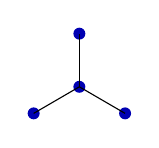
\begin{tikzpicture}[baseline=0pt, scale=1.35]
\fill[blue!70!black] (0,0) circle (1.6pt);
\fill[blue!70!black] (0,0.5) circle (1.6pt);
\fill[blue!70!black] (0.43,-0.25) circle (1.6pt);
\fill[blue!70!black] (-0.43,-0.25) circle (1.6pt);
\draw[thin] (0,0) -- (0,0.5);
\draw[thin] (0,0) -- (0.43,-0.25);
\draw[thin] (0,0) -- (-0.43,-0.25);
\end{tikzpicture}\\[3pt]{\small Tri.+centre, 8~m}} &
\parbox{2.3cm}{\centering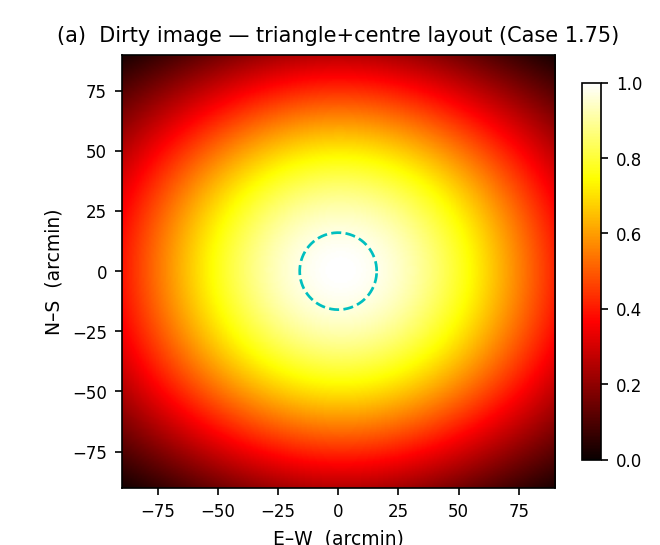
\includegraphics[width=\linewidth]{figs/fig_case175_dirty_crop.png}} &
\textbf{Case 1.75.} Same 4 antennas, DLITE-inspired triangle$+$centre~\cite{helmboldt2021dlite}: all 6 baselines point in distinct directions
$\Rightarrow$ N-S FWHM $19.8'$ ($\mathbf{9.1\times}$ better). \\
\bottomrule
\end{tabular}

\centering\normalsize\textbf{Same 4 antennas throughout --- placement,
not antenna count, is what improves resolution.}
\end{minipage}%
\end{frame}

\begin{frame}{\ftitle{Sensitivity and Burst Detectability}}
\footnotesize
\begin{itemize}
  \setlength{\itemsep}{5pt}
  \item Minimum detectable flux $\Delta S_{\min}\approx0.026$--$0.183$~sfu,
  depending on the number of integration dumps averaged.
  \item Quiet-Sun detection SNR $>500{:}1$ across every array
  configuration tested.
  \item Type~II/III bursts exceed the noise floor by
  $\mathbf{10^{4}\text{--}10^{5}\times}$.
\end{itemize}
\vspace{6pt}
\small $\Rightarrow$ The system is not limited by thermal noise but by
$(u,v)$-coverage --- the burst science goal from the introduction is
fully achievable with this hardware. \emph{(Per-sample SNR and ADC
headroom detail in backup.)}
\end{frame}

% ============================================================
\section{Diagnosis}

\begin{frame}{\ftitle{Closing the Loop: Diagnosing the Field Trial}}
\footnotesize
Back to the Xuan Mai trial from the introduction. Comparing the simulator
against a real 2-antenna analogue trace measured the same day
(20~March~2025) isolates \textbf{two} confirmed, quantifiable causes:
\vspace{4pt}
\begin{columns}[t]
\column{.48\textwidth}
\begin{block}{\centering Uncalibrated receiver chain}
\footnotesize
\centering
Measured solar excess is \textbf{23.8$\times$} below the simulated
prediction $\Rightarrow$ effective $T_{\rm sys}\approx3600$~K, not the
150~K assumed --- the LNA chain was never calibrated in the field.
\end{block}
\column{.48\textwidth}
\begin{block}{\centering Clock incoherence}
\footnotesize
\centering
A typical RTL-SDR crystal drifts $\sim$1~ppm $\Rightarrow$ coherence
time $\approx1.6$~ms at 610~MHz --- four orders of magnitude shorter
than the 43.2~s dump. Fringe amplitude collapses to zero
\textbf{regardless of SNR}.
\end{block}
\end{columns}
\vspace{8pt}
\begin{alertblock}{Takeaway}
\small The field failure was \textbf{not} a concept failure: it reduces
to two fixable hardware requirements --- calibrate $T_{\rm sys}$, and
add a GPS-disciplined (or shared 10~MHz reference) clock.
\end{alertblock}
\end{frame}

% ============================================================
\section{Conclusion}

\begin{frame}{\ftitle{Conclusion \& Future Work}}
\begin{block}{\cmark\ 1. A trustworthy physics simulator}
\footnotesize
4NEC2 antenna model cross-checked against direct NanoVNA measurement;
mutual coupling confirms antennas act as independent sensors; simulated
visibility, fringe, and imaging all match analytic theory on real solar
flux data.
\end{block}
\vspace{4pt}
\begin{block}{\cmark\ 2. Optimized antenna placement}
\footnotesize
Same 4-antenna hardware, three geometries tested: E-W line $\to$ cross
$\to$ DLITE-inspired triangle gives a \textbf{9.1$\times$} N-S
resolution gain from \emph{rearrangement alone}.
\end{block}
\vspace{6pt}
\begin{block}{Future Work}
\footnotesize
\begin{itemize}
  \item FPGA hardware correlator, hardware-in-the-loop fringe validation.
  \item Physical DLITE-inspired array upgrade at Xuan Mai, with a
  calibrated LNA chain and GPS-disciplined clock.
  \item Recorded Type~II/III burst input, CLEAN
  deconvolution~\cite{hogbom1974}, real-time operation.
\end{itemize}
\end{block}
\end{frame}

% ============================================================
% Backup slides: advance the section counter (for \ftitle numbering)
% without adding a "Backup" entry to the Table of Contents.
\stepcounter{section}

\begin{frame}{\ftitle{Backup: Key Contributions}}
\begin{enumerate}
  \item \textbf{A validated antenna model:} the low-cost commercial
  Yagi-Uda is cross-checked against direct NanoVNA measurement, plus a
  mutual coupling study proving the elements act independently at every
  operating baseline.
  \item \textbf{A general end-to-end interferometry engine:} one
  $(u,v,w)$ formulation, reused consistently for per-antenna phase,
  baseline projection, and fringe stopping, valid for \emph{any} 2-D
  array layout.
  \item \textbf{Validation with real data:} driven by real Learmonth
  610~MHz flux, the pipeline reproduces \textbf{three} classical
  aperture-synthesis signatures \emph{simultaneously} --- fringe period,
  jinc visibility, dirty-image consistency.
  \item \textbf{A structured comparison against APSYNSIM:} real data,
  real antenna beam, physics-based noise, and an FPGA hardware path ---
  four concrete advantages over the standard teaching tool.
  \item \textbf{A single reproducible workflow:} raw SWS flux file
  $\to$ calibrated dirty image in under two minutes, every parameter in
  one configuration cell.
\end{enumerate}
\end{frame}

\begin{frame}{\ftitle{Backup: Solar Radio Bursts, Types I--V}}
\begin{columns}[c]
\column{.55\textwidth}
\begin{itemize}
  \footnotesize
  \item Superimposed on the quiet-Sun thermal background, transient bursts can
  raise the flux by \textbf{orders of magnitude}.
  \item \textbf{Type I}: long-lived, narrowband noise storms.
  \item \textbf{Type III}: fast-drifting, electron beams on open field lines
  --- dominant at decimetre wavelengths.
  \item \textbf{Type II}: slowly drifting, traces coronal shock fronts (CMEs).
  \item \textbf{Type IV}: broadband continuum following flares.
  \item \textbf{Type V}: brief continuum sometimes following Type~III
  bursts, tracing trapped electron streams.
\end{itemize}
\column{.45\textwidth}
\centering
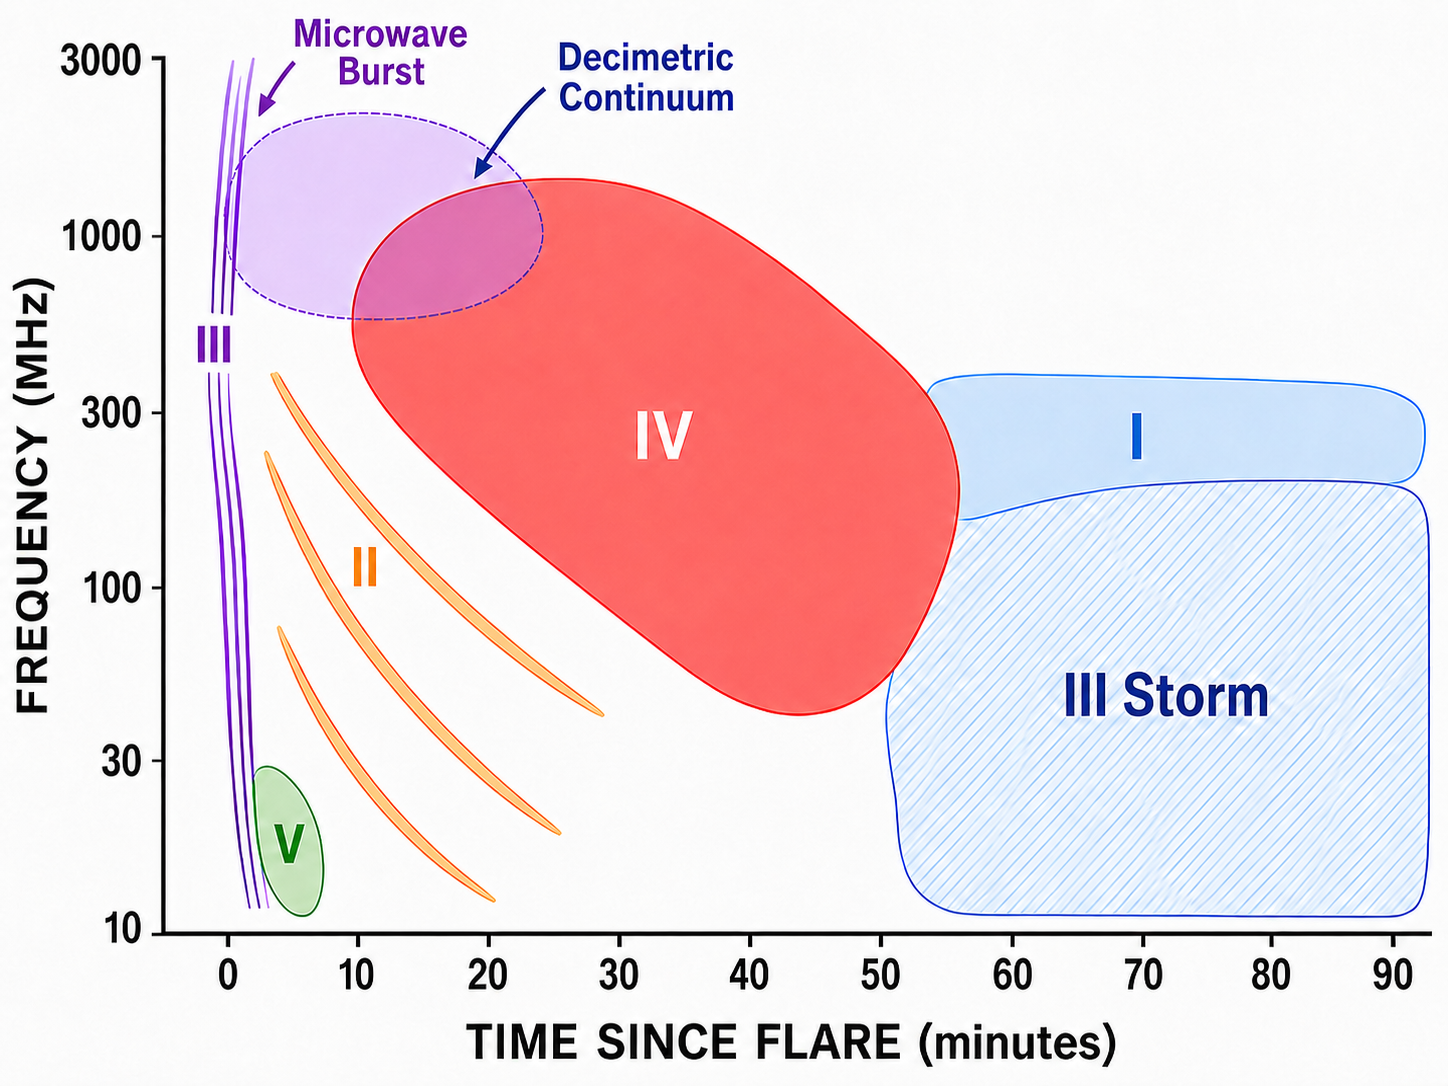
\includegraphics[width=\linewidth]{figs/fig_solar_dynamic_spectrum.png}
\end{columns}
\vspace{4pt}
\small Adapted from McLean \& Labrum and Dulk~\cite{dulk1985}.
\end{frame}

\begin{frame}{\ftitle{Backup: The Idea of Interferometry, Step by Step}}
\centering
\setlength{\tabcolsep}{2pt}
\begin{tabular}{ccc}
\parbox{.3\linewidth}{\centering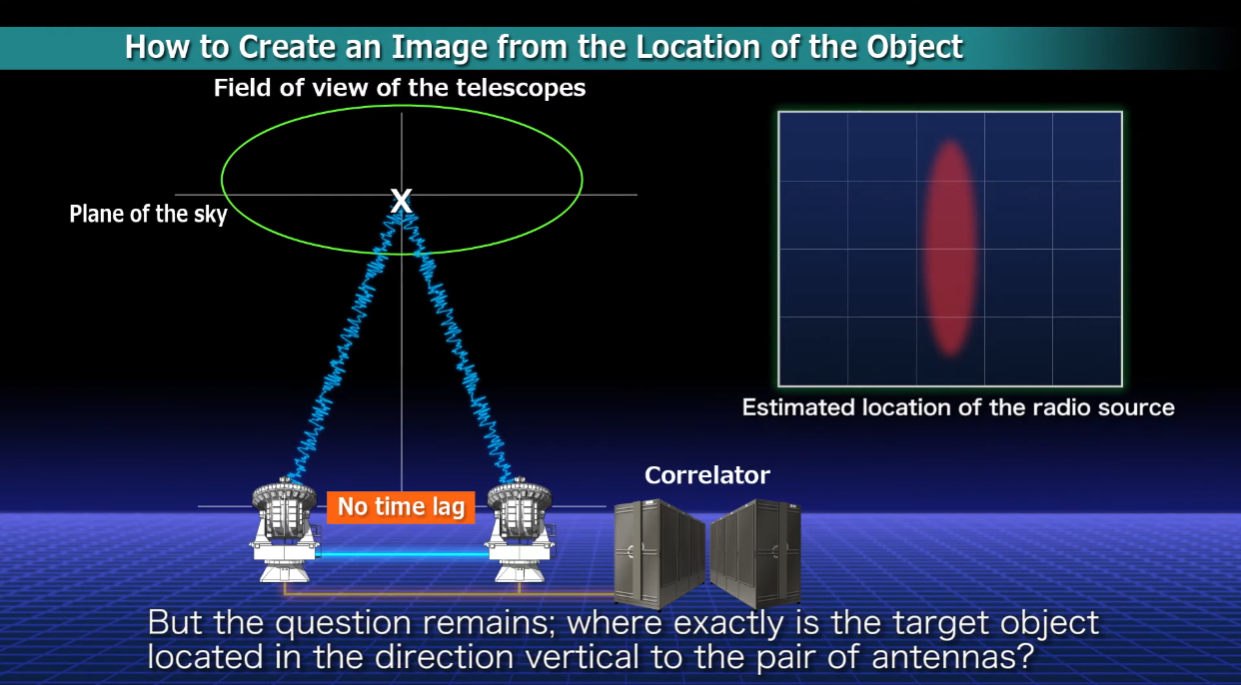
\includegraphics[width=\linewidth]{figs/fig_interf_1_notimelag.png}\\[2pt]\scriptsize 1. Two antennas, source dead ahead: no time lag.} &
\parbox{.3\linewidth}{\centering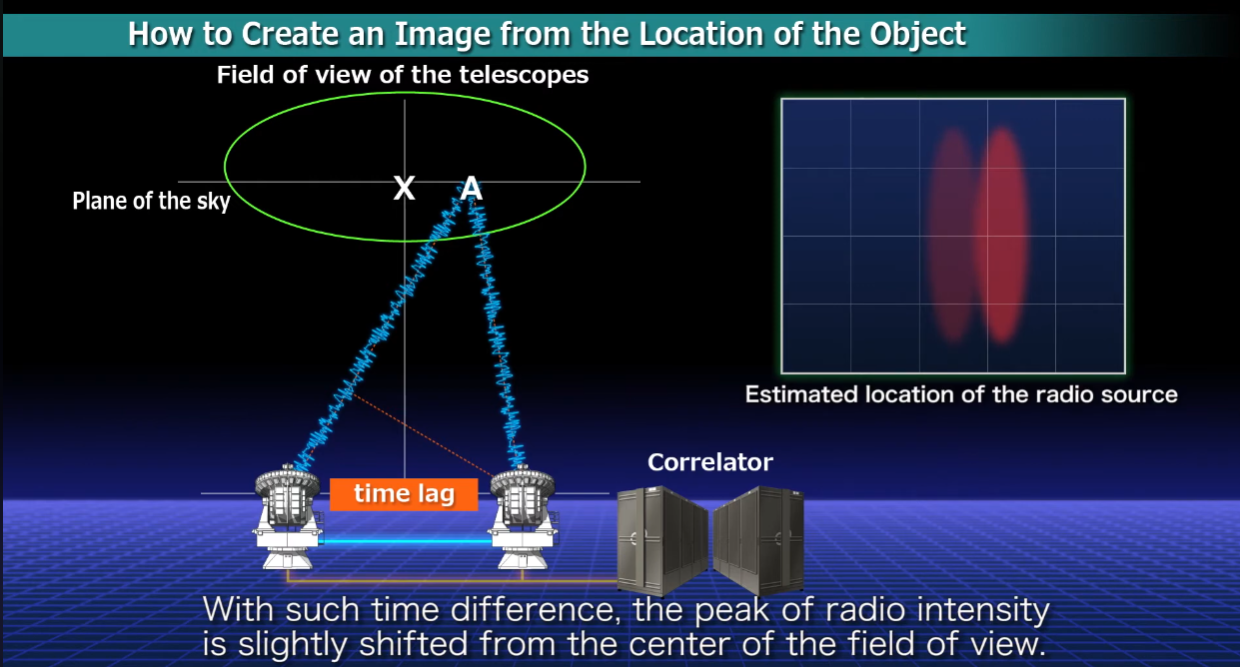
\includegraphics[width=\linewidth]{figs/fig_interf_2_timelag.png}\\[2pt]\scriptsize 2. Source off to one side: a tiny time lag appears.} &
\parbox{.3\linewidth}{\centering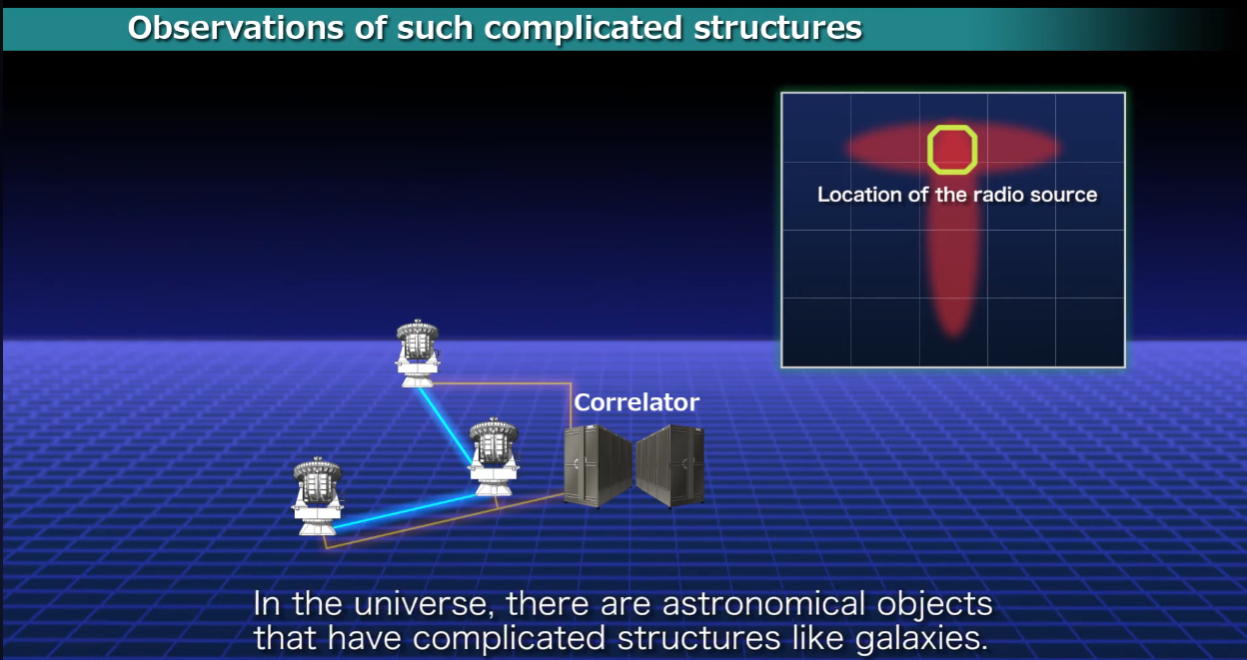
\includegraphics[width=\linewidth]{figs/fig_interf_3_threeant.png}\\[2pt]\scriptsize 3. A real source isn't one point --- need more.} \\[8pt]
\parbox{.3\linewidth}{\centering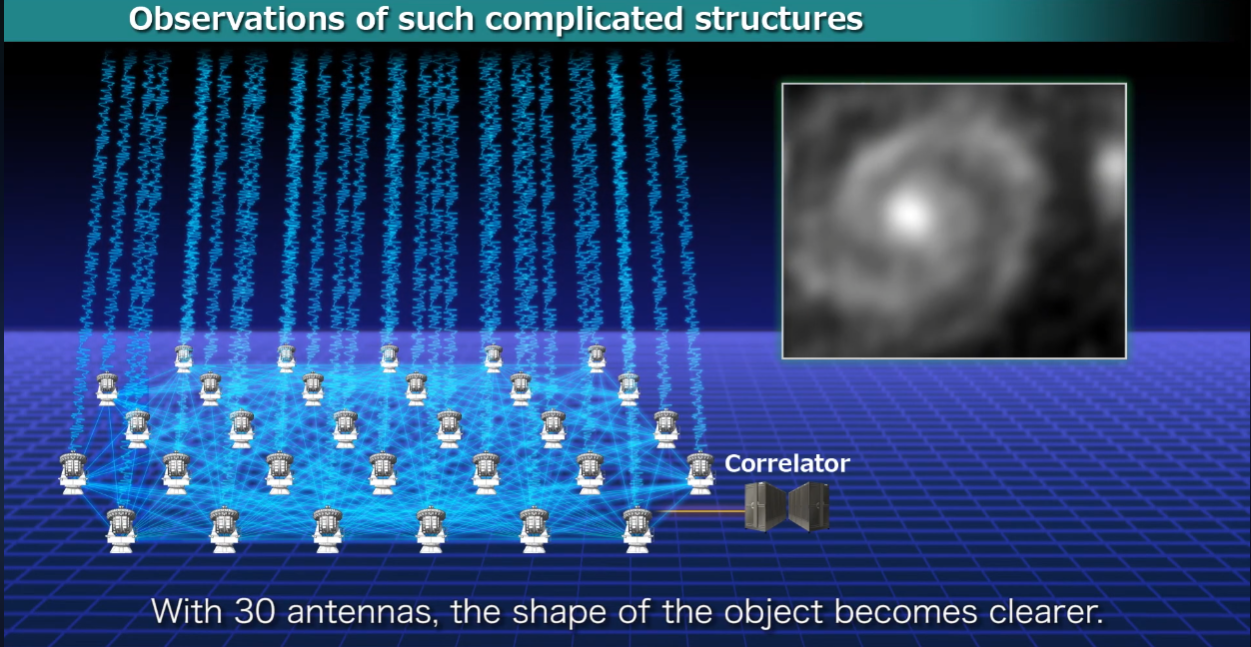
\includegraphics[width=\linewidth]{figs/fig_interf_5_30ant.png}\\[2pt]\scriptsize 5. With 30 antennas, the shape becomes clear.} &
\parbox{.3\linewidth}{\centering\Large$\Longleftarrow$} &
\parbox{.3\linewidth}{\centering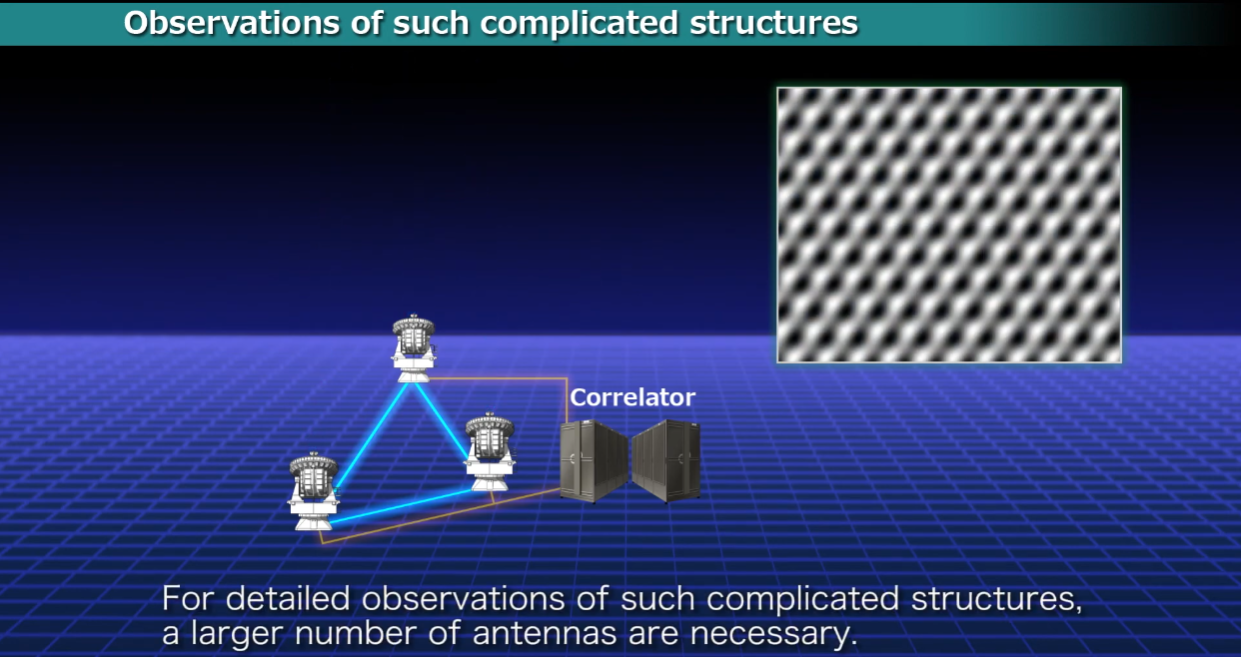
\includegraphics[width=\linewidth]{figs/fig_interf_4_fringepattern.png}\\[2pt]\scriptsize 4. Just 3 antennas: only a coarse, striped pattern.}
\end{tabular}
\vspace{4pt}

\small Each pair of antennas measures one time lag $\Rightarrow$ one
piece of the picture. \textbf{More antennas, more pairs, sharper image.}
\end{frame}

\begin{frame}{\ftitle{Backup: 3-D Radiation Pattern \& E-plane}}
\begin{columns}[c]
\column{.48\textwidth}
\centering
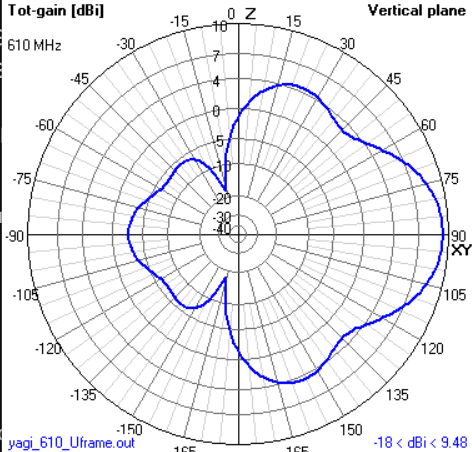
\includegraphics[width=\linewidth]{figs/fig_pattern_eplane_crop.png}\\
\small Simulated E-plane (vertical) pattern, 610~MHz (4NEC2).
\column{.48\textwidth}
\centering
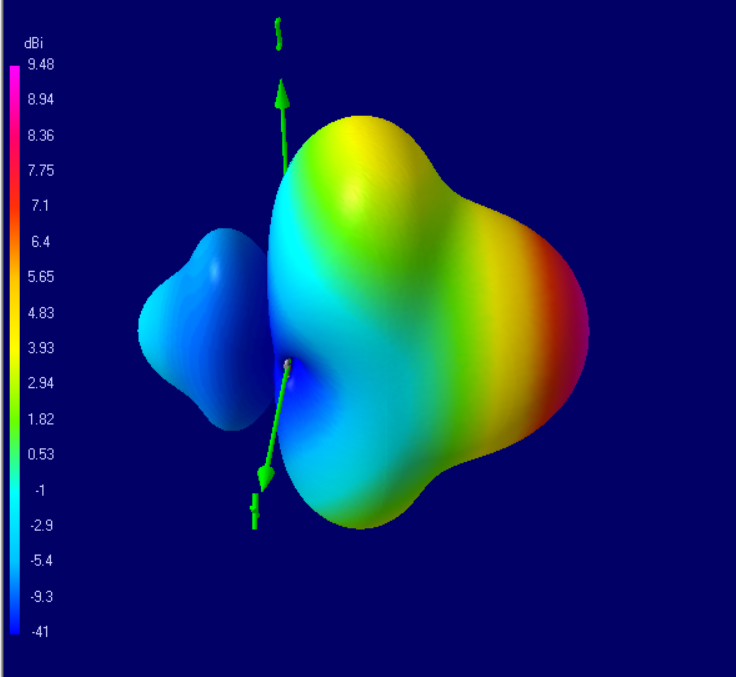
\includegraphics[width=\linewidth]{figs/fig_3d_radiation_pattern.png}\\
\small 3-D directivity pattern at 610~MHz.
\end{columns}
\vspace{4pt}
\footnotesize Directional gain toward the horizon --- well matched to a
low-elevation solar transit at Learmonth's latitude.
\end{frame}

\begin{frame}{\ftitle{Backup: Full Input \& Voltage Synthesis}}
\centering
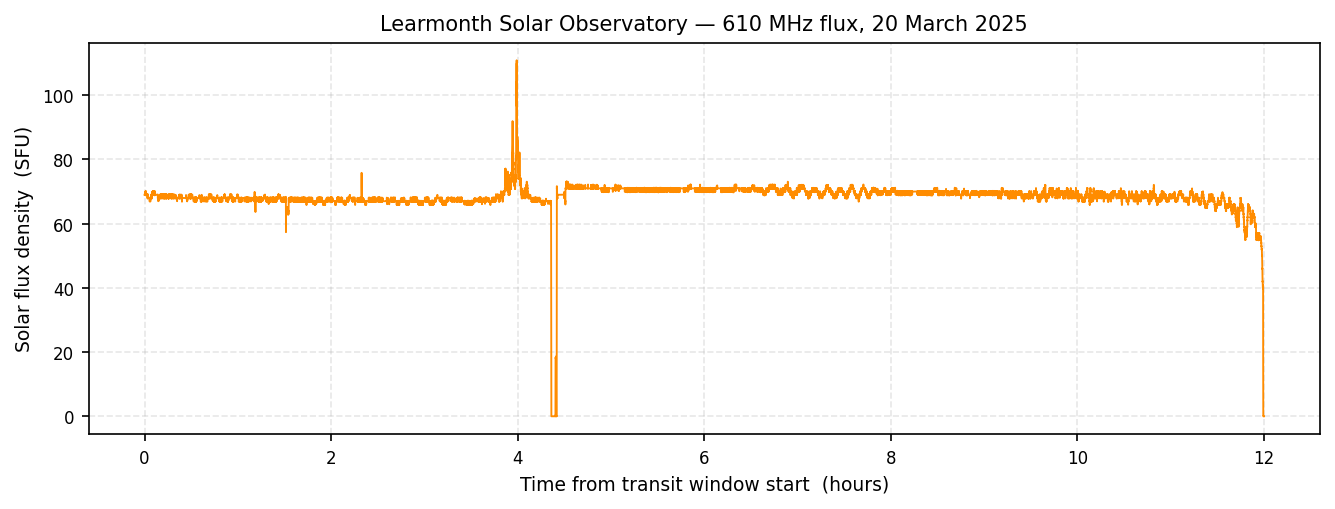
\includegraphics[width=0.62\linewidth]{figs/fig_sws_flux_day.png}\\[1pt]
{\scriptsize $\Downarrow$ Friis $+$ 4NEC2 pattern $+$ \mbox{Johnson--Nyquist} noise}\\[1pt]
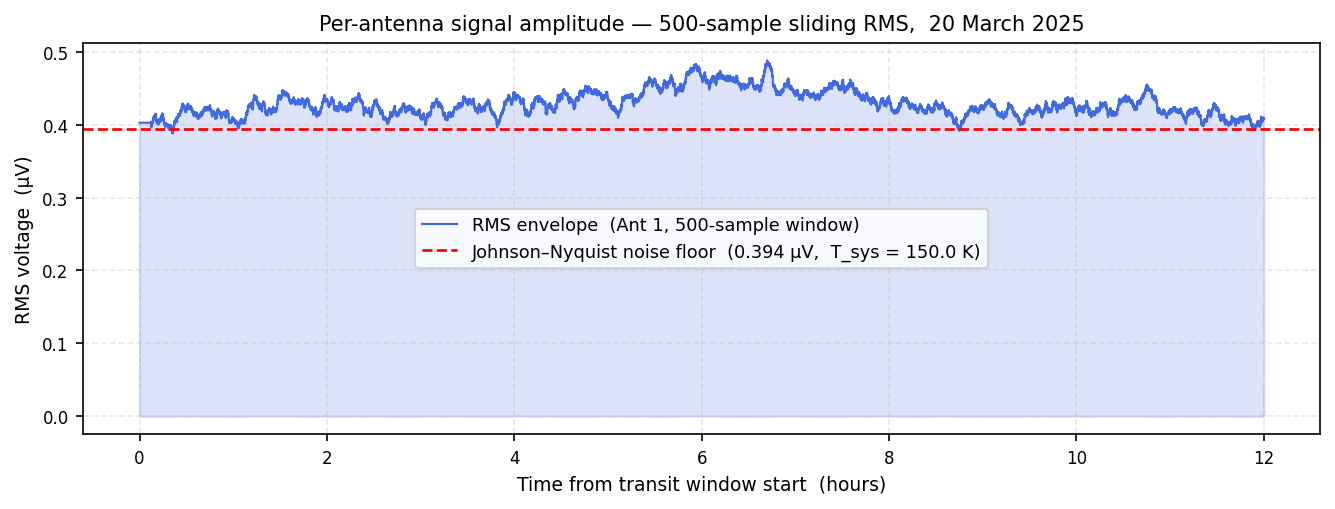
\includegraphics[width=0.62\linewidth]{figs/fig_voltage_env.png}

\vspace{1pt}
\begin{itemize}
  \footnotesize
  \item \textbf{Top:} real, archived, already-calibrated 610~MHz flux
  from SWS Learmonth, Australia~\cite{sws} (20 March 2025).
  \item \textbf{Bottom:} the same track after Friis power conversion,
  the 4NEC2 primary beam, and additive noise --- per-antenna complex
  baseband voltage, ready for correlation.
\end{itemize}
\end{frame}

\begin{frame}{\ftitle{Backup: Array Geometry, Site \& Observing Setup}}
\centering
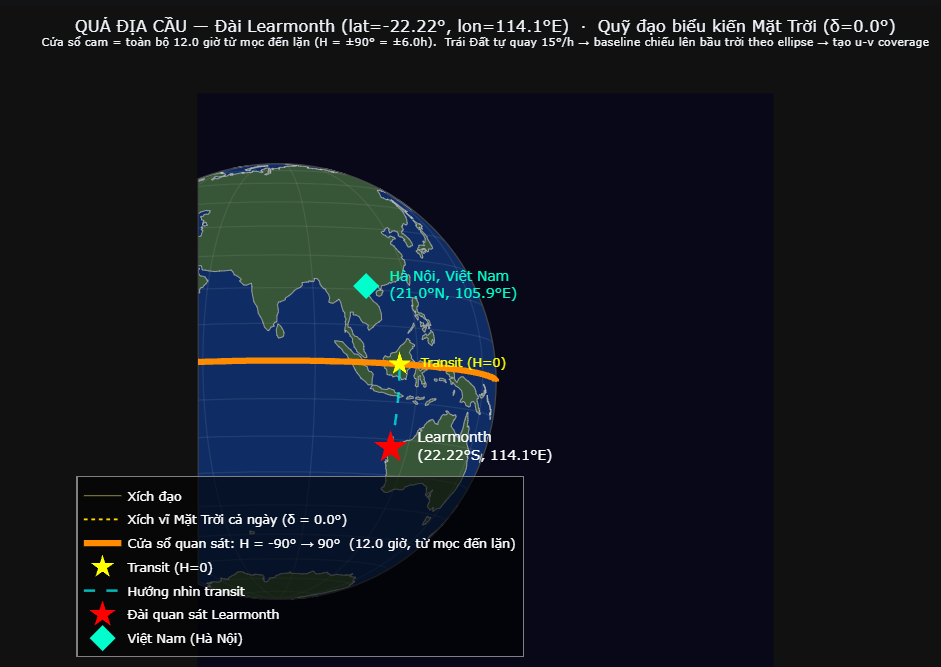
\includegraphics[width=0.65\linewidth]{figs/fig_globe_track.png}

\vspace{4pt}
\begin{itemize}
  \footnotesize
  \item Learmonth Observatory, site latitude $-22.2^\circ$; the Sun
  transits within hour angle $H\in[\pm90^\circ]$, a 12-hour observing
  window.
  \item Ground positions (East-North-Up) are rotated first by site
  latitude, then by the Sun's current hour angle and declination, to
  give every baseline's $(u,v,w)$ in wavelengths at every
  instant~\cite{tms2017}.
\end{itemize}
\end{frame}

\begin{frame}{\ftitle{Backup: Mutual Coupling Curve}}
\centering
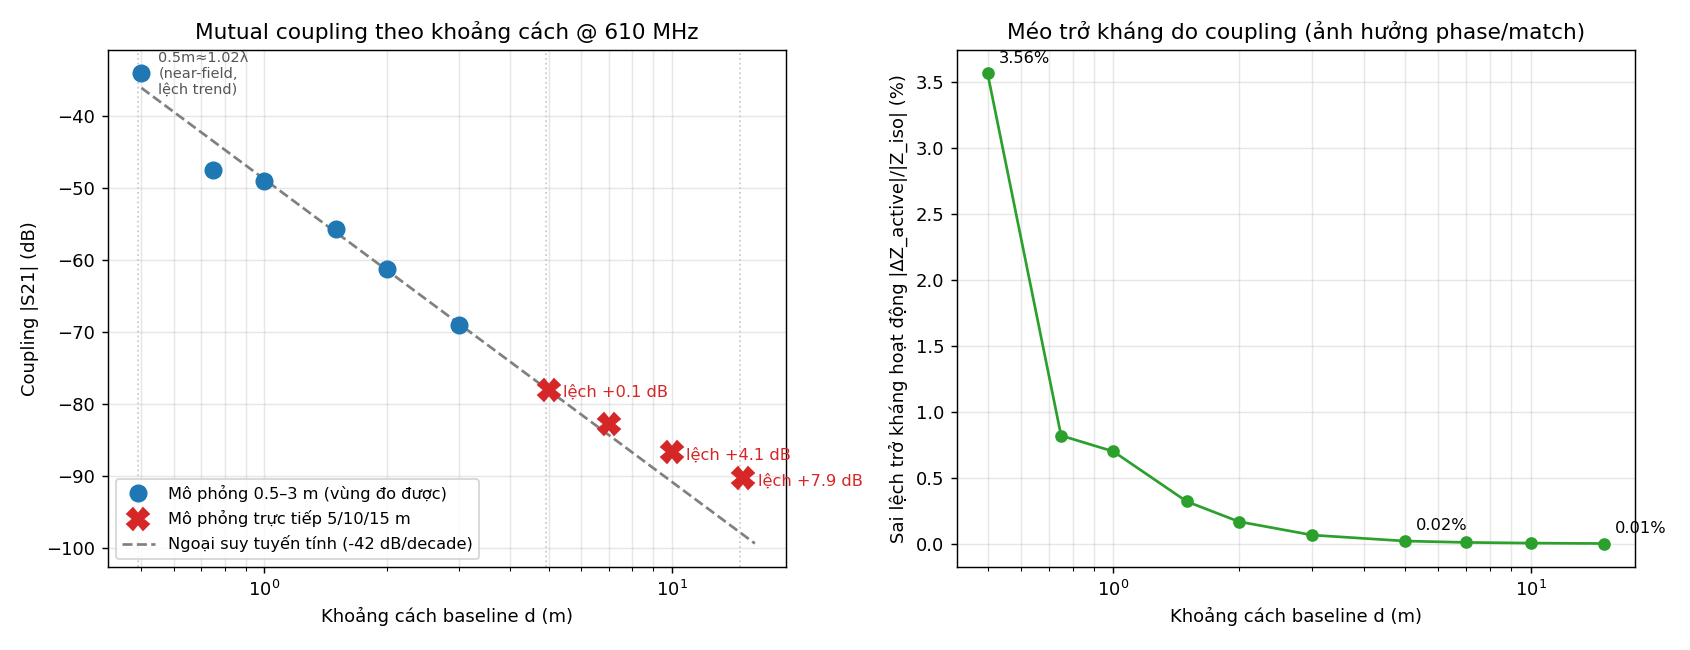
\includegraphics[width=0.98\linewidth]{figs/fig_coupling_curve.png}

\footnotesize
\begin{itemize}
  \setlength{\itemsep}{1pt}
  \item \textbf{Left:} coupling $|S_{21}|$ vs.\ baseline distance ---
  measured 0.5--3~m (circles), simulated directly at 5/10/15~m (crosses).
  Falls below $-78$~dB by 5~m, $-87$~dB by 10~m.
  \item \textbf{Right:} the impedance distortion that coupling causes on
  each active element --- already $<0.02\%$ by 5~m.
  \item[$\Rightarrow$] Both views agree: antennas behave as
  \textbf{independent sensors} at the operating baselines used in this
  thesis (8~m and above); no Jones-matrix cross-coupling correction is
  needed.
\end{itemize}
\end{frame}

\begin{frame}{\ftitle{Backup: Position Matrix --- Computing $(u,v,w)$}}
\footnotesize
\textbf{Step 1 --- local to equatorial} (rotate by site latitude
$\varphi$):
\[
\begin{pmatrix}X\\Y\\Z\end{pmatrix} =
\begin{pmatrix}
-\sin\varphi & 0 & \cos\varphi\\
0 & 1 & 0\\
\cos\varphi & 0 & \sin\varphi
\end{pmatrix}
\begin{pmatrix}E\\N\\U\end{pmatrix}
\]
\textbf{Step 2 --- equatorial to baseline} (rotate by hour angle $H$,
declination $\delta$ of the source):
\[
\begin{pmatrix}u\\v\\w\end{pmatrix} =
\begin{pmatrix}
\sin H & \cos H & 0\\
-\sin\delta\cos H & \sin\delta\sin H & \cos\delta\\
\cos\delta\cos H & -\cos\delta\sin H & \sin\delta
\end{pmatrix}
\begin{pmatrix}X\\Y\\Z\end{pmatrix}
\]
\begin{itemize}
  \setlength{\itemsep}{2pt}
  \item Each antenna's ground position (East-North-Up) is rotated first
  by \textbf{where the array sits} on Earth ($\varphi$, fixed), then by
  \textbf{where the Sun is right now} ($H,\delta$, time-varying)
  ~\cite{tms2017}.
  \item Same two matrices, reused everywhere: per-antenna phase (Stage~1)
  and baseline $(u,v,w)$ coordinates for every antenna pair (Stage~3).
  \item As hour angle $H$ changes through the day, each baseline traces
  an arc in the $(u,v)$ plane --- this is Earth-rotation synthesis.
\end{itemize}
\end{frame}

\begin{frame}{\ftitle{Backup: Beyond 4 Antennas (Case 2)}}
\centering
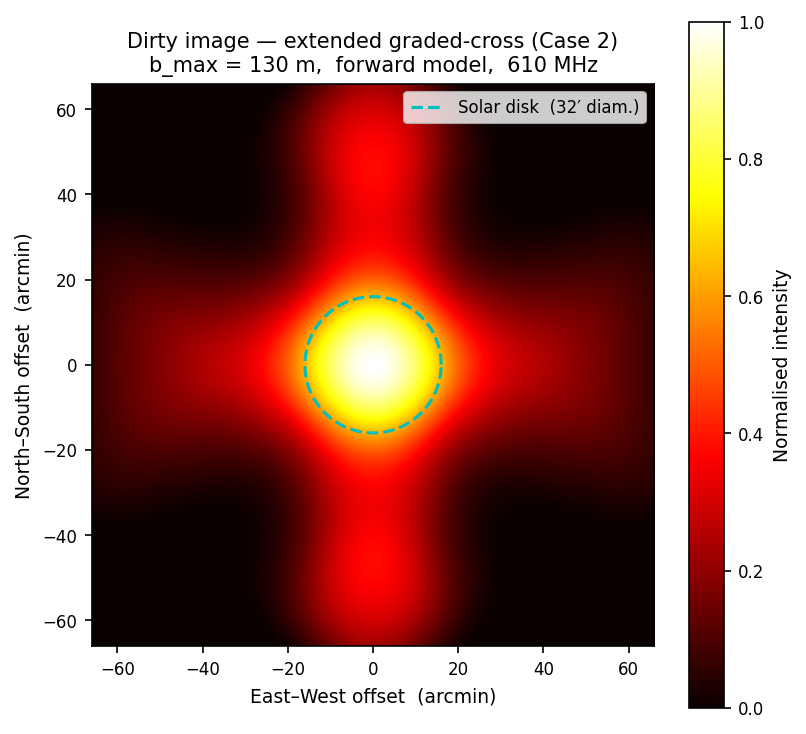
\includegraphics[width=0.36\linewidth]{figs/fig_case2_image.png}

\footnotesize
\begin{itemize}
  \setlength{\itemsep}{1pt}
  \item Unlike Cases 1/1.5/1.75, \textbf{not} the same 4-antenna
  hardware --- a separate 17-element graded 2-D cross (1 centre $+$ 4
  arms $\times$ 4 radii: 5/15/35/65~m), forward-modelled (idealised
  uniform-disk sky, no noise).
  \item Baselines out to 130~m ($\approx264\,\lambda$ --- past the
  $\approx132\,\lambda$ visibility null from Sec.~4.1) $\Rightarrow$
  E-W resolution $\approx11'$, beginning to resolve the $32'$ disk.
  \item[$\Rightarrow$] A separate design question: \emph{if} more
  antennas become available, a graded 2-D array like this is what
  starts to resolve the disk itself, not just detect it.
\end{itemize}
\end{frame}

\begin{frame}{\ftitle{Backup: Full Array Sweep (5 Layouts)}}
\centering
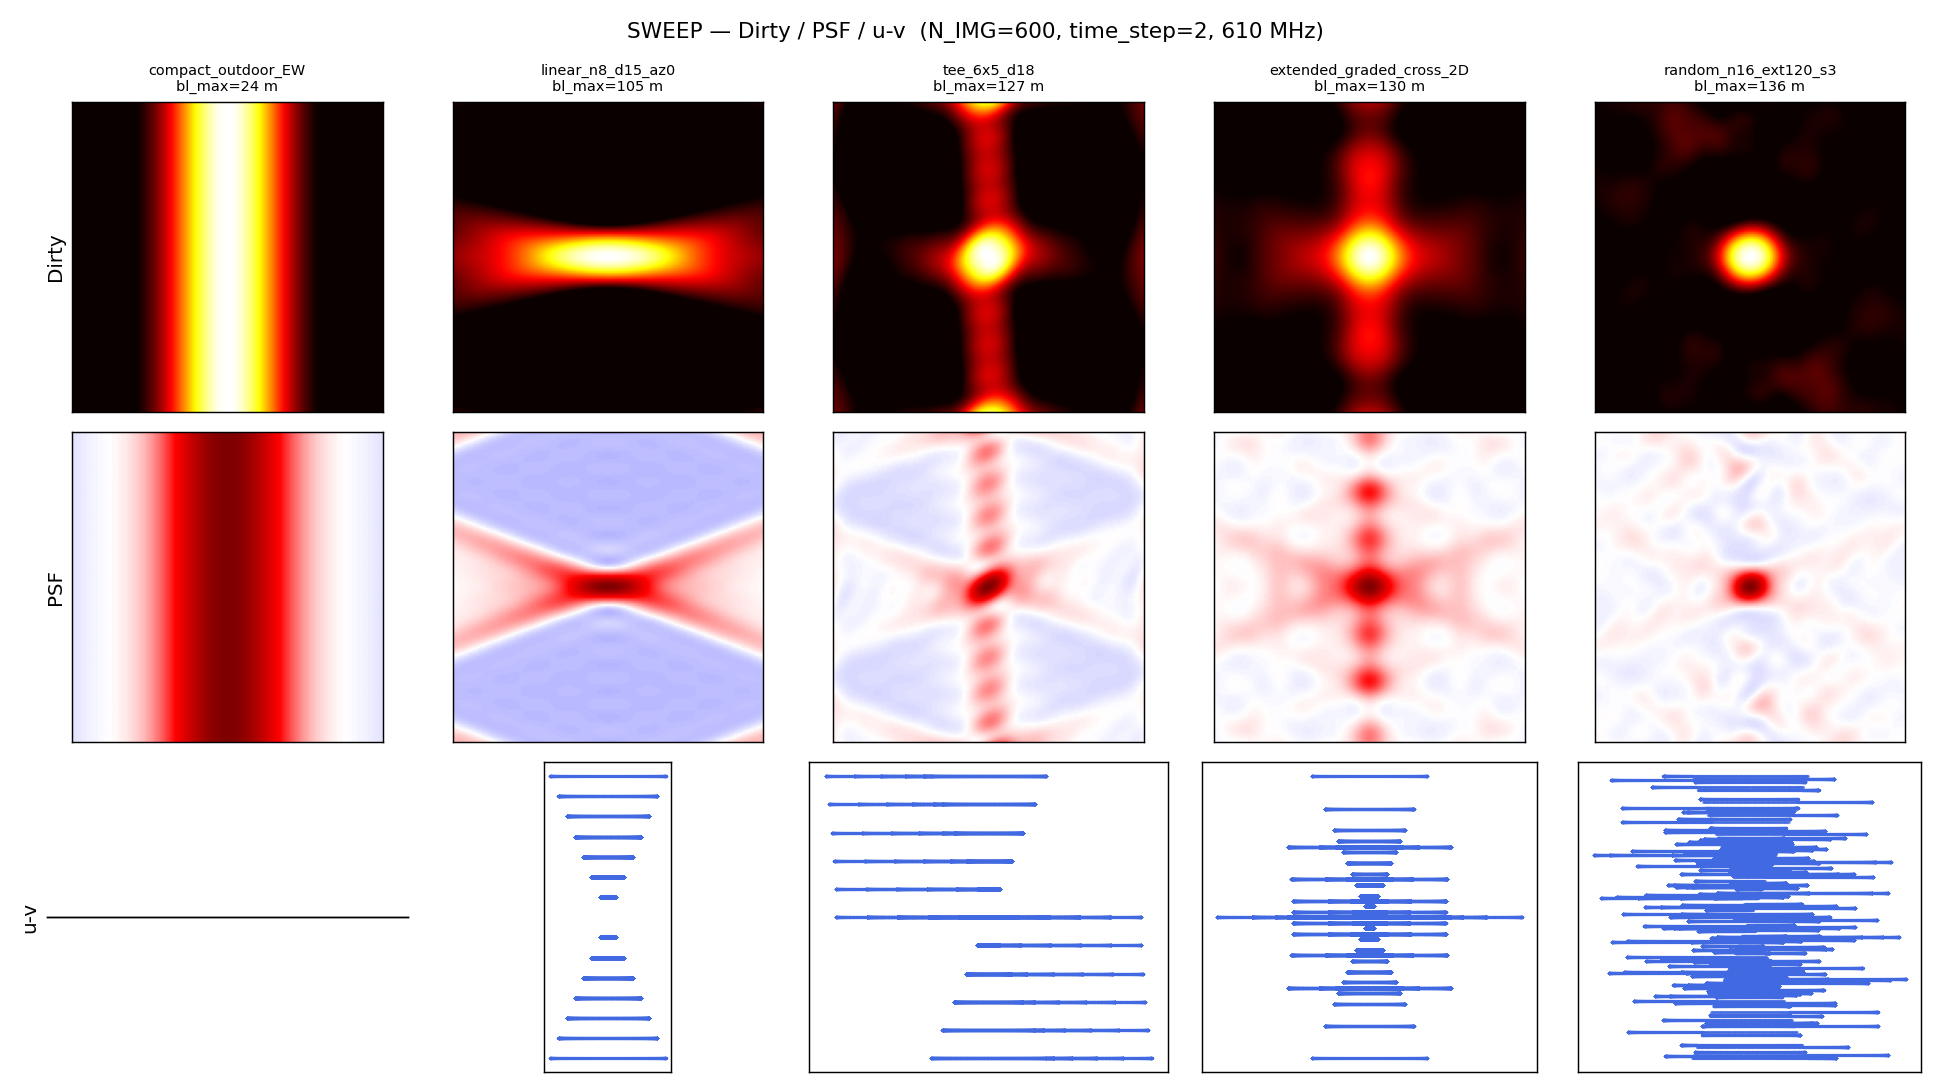
\includegraphics[width=0.85\linewidth]{figs/fig_layout_sweep.png}
\footnotesize Five candidate layouts, same simulator --- compact E--W,
linear, tee, extended graded cross, and random. \textbf{Top:} dirty
image; \textbf{middle:} PSF; \textbf{bottom:} $(u,v)$ coverage.
\end{frame}

\begin{frame}{\ftitle{Backup: Johnson--Nyquist Noise Model}}
\footnotesize
Thermal noise added to every simulated antenna voltage sample (Engine~A):
\[
P_{\text{noise}} = k_B\,T_{\text{sys}}\,B
\qquad
V_{\text{noise}} = \sqrt{P_{\text{noise}}\,R_{\text{load}}}
\qquad
\sigma_{\text{noise}} = \frac{V_{\text{noise}}}{\sqrt{2}}
\]
\centering
\begin{tabular}{clc}
\toprule
Symbol & Meaning & Value used \\
\midrule
$k_B$ & Boltzmann constant & $1.381\times10^{-23}$~J/K \\
$T_{\text{sys}}$ & Assumed system noise temperature & 150~K \\
$B$ & Receiver bandwidth & 1~MHz \\
$R_{\text{load}}$ & Antenna output load impedance & 75~$\Omega$ \\
$\sigma_{\text{noise}}$ & Per-quadrature (I/Q) noise std.\ dev. & $\approx0.28~\mu$V \\
\bottomrule
\end{tabular}
\vspace{6pt}
\raggedright
\begin{itemize}
\setlength{\itemsep}{2pt}
  \item $\sigma_{\text{noise}}$ is the value actually added to each simulated
  voltage sample; the $\sqrt{2}$ split is because total noise power is shared
  equally between the real and imaginary (I/Q) components.
  \item $T_{\text{sys}}=150$~K is a \textbf{design assumption} (uncalibrated
  receiver chain), not a measurement --- the Xuan Mai field trial found the
  real value $\approx3600$~K (Sec.~6.1), which is why field SNR fell far
  short of this model.
  \item[$\Rightarrow$] This noise floor is the denominator behind every
  SNR/sensitivity figure quoted in Sec.~5.3 and the next backup slide.
\end{itemize}
\end{frame}

\begin{frame}{\ftitle{Backup: Sensitivity Detail}}
\footnotesize
\centering{\scriptsize SEFD (System Equivalent Flux Density) --- the
source flux that would equal the receiver's own noise power; smaller
SEFD $=$ more sensitive receiver.}
\raggedright
\[
\underbrace{\text{SEFD}}_{\text{sfu}} = \frac{2k_BT_{\text{sys}}}{A_{\text{eff}}}
= \frac{2(1.381\times10^{-23})(150)}{1705\times10^{-4}}
\approx 243~\text{sfu}
\]
\[
\Delta S_{\min} = \frac{\text{SEFD}}{\sqrt{2B\tau}}
\;\;\Rightarrow\;\;
\begin{cases}
\tau=0.864~\text{s (1 sample)}: & \dfrac{243}{\sqrt{2(10^6)(0.864)}}\approx0.183~\text{sfu}\\[6pt]
\tau=43.2~\text{s (1 dump)}: & \dfrac{243}{\sqrt{2(10^6)(43.2)}}\approx0.026~\text{sfu}
\end{cases}
\]
\[
\text{SNR}_{\text{quiet-Sun}} = \frac{S_{\text{quiet}}}{\Delta S_{\min}}
= \frac{68~\text{sfu}}{0.026~\text{sfu}} \approx 2600 \;\;(\gg 500{:}1)
\]
\vspace{4pt}
\centering
ADC headroom: noise floor occupies $>20$ LSBs (Least Significant
Bits --- the smallest step size of the 16-bit sample) $\Rightarrow$
noise is not lost to rounding, ready for an FPGA correlator.
\end{frame}

% ============================================================
\begin{frame}[allowframebreaks]
\frametitle{References}
\tiny{
\bibliography{refs_slides}
}
\end{frame}

\begin{frame}
\Huge{\centerline{Thank you!}}
\end{frame}

\end{document}
